\documentclass[12p,english]{article}
\usepackage{graphicx} % Required for inserting images
\usepackage{algorithm}
\usepackage{algpseudocode}
\usepackage{amsmath}
\usepackage{amsthm}
\usepackage{float}

\title{\textbf{Parallelized Matrix-Matrix \\\medskip Multiplication With CUDA}\\
Advanced Methods for Scientific Computing }
\author{Abril Cano Castro \\ abril.cano@mail.polimi.it}
\date{}

\begin{document}

\maketitle

\section{Introduction}

Matrix multiplication involves the multiplication of individual elements from two matrices to produce a new matrix. While the operation may seem straightforward, its significance is undeniable as it is involved in an immense quantity of tasks performed daily. 
This operation as the core of linear algebra, plays a fundamental role in a wide range of scientific and engineering applications. It is used to solve systems of linear equations, compute derivatives and integrals, and perform data analysis tasks. In recent years, the increasing complexity of scientific simulations and the demand for real-time data processing have fueled the need for efficient parallel algorithms for matrix multiplication. The efficiency of matrix multiplication is crucial for these applications, as it can significantly impact the overall computational time and performance, and therefore the complexity and range of problems that can be solved. 


\section{Naive Matrix Matrix Multiplication}

The basic matrix matrix multiplication algorithm as proposed in mathematics states that given to matrices say $A$ of dimensions $m \times n$ and $B$ of dimensions $n \times p $ the resulting matrix $C$ of dimensions $m \times p$ is obtained by computing the elements $C[i][j]$ as the sum of the products corresponding elements from the $i$-th row of matrix $A$ and the $j$-th column of matrix $B$. This operation is succinctly expressed by the formula:\[ C[i][j] = \sum_{k=1}^{n} A[i][k] \cdot B[k][j] \]
This algorithm follows a nested loop structure, iterating over each element of the resulting matrix $C$. The efficiency of this method is contingent upon the matrix dimensions, with a time complexity of $O(m \cdot n \cdot p)$ and can be implemented as follows. 

\begin{algorithm}
\begin{algorithmic}[1]
\Procedure{MatrixMultiplication}{Matrix $A$, Matrix $B$}
    \For{$i \gets 1$ to $\text{rows}(A)$}
        \For{$j \gets 1$ to $\text{columns}(B)$}
            \State $C[i][j] \gets 0$ \Comment{Initialize result matrix}
            \For{$k \gets 1$ to $\text{columns}(A)$}
                \State $C[i][j] \gets C[i][j] + A[i][k] \times B[k][j]$
            \EndFor
        \EndFor
    \EndFor
\EndProcedure
\end{algorithmic}

\caption{{Naive Matrix-Matrix Multiplication}}
\end{algorithm}

Despite its mathematical simplicity,seems evident the barrier that the utilization this method introduces.Dealing with large matrices did not seem feasible at first because the computational complexity that grows cubically with the dimensions of the matrices involved. Even modern CPUs become insufficient when dealing with the millions of matrix-matrix multiplications that are necessary to solve current technological and mathematical problems. 

To overcome this limitation more sophisticated and efficient methods were introduced to perform this operation. Strategies such as unrolling the loops, performing cache aware operations, SIMD vectorization (Single Instruction Multiple Data), and thread parallelization were implemented to improve the performance of this operation, and despite being quite successful the continuous growth of the dimensions achieved called for more powerful tools. 

\section{Graphic Processing Units for Matrix-Matrix Multiplication}
Graphics Processing Units (GPUs), originally designed for rendering graphics in video games, have evolved into powerful accelerators for general-purpose computation. Their parallel architecture, comprising thousands of cores capable of simultaneously executing numerous threads, makes GPUs highly suitable for computationally intensive tasks. In the realm of general-purpose computing, GPUs excel in parallelizing tasks that exhibit data parallelism, such as matrix multiplications, image processing, and machine learning algorithms. By offloading parallelizable computations to the GPU, significant speedups can be achieved compared to traditional Central Processing Units (CPUs). Unlike CPUs, which are optimized for single-threaded performance, GPUs can handle a massive number of parallel operations concurrently, greatly increasing throughput. 
Taking this into account this operation was the perfect candidate to take advantage of all the power introduced by this computational tools as it is a task that can be highly parallelizable. With the development and application of this technology performing multiplications of matrices of large dimensions.

\section{CUDA}
CUDA, or Compute Unified Device Architecture, is a parallel computing platform and programming model developed by NVIDIA for their Graphics Processing Units (GPUs). Introduced in 2007, CUDA enables developers to harness the immense parallel processing power of NVIDIA GPUs to accelerate general-purpose computations. It allows programmers to write code that can be executed on the GPU, taking advantage of the many cores to perform thousands of parallel operations simultaneously. CUDA provides a set of extensions to the C programming language, making it accessible to a broad audience of developers.


In CUDA, parallel computations are orchestrated through the use of kernels, which are functions designed to be executed in parallel on the GPU. The execution of a kernel is initiated by the host CPU and involves the creation of a grid of thread blocks. Each thread block consists of multiple threads, and the entire grid is organized in a three-dimensional manner. The number of threads in each block and the number of blocks in the grid can be specified when launching the kernel.
When a kernel is launched, the GPU scheduler assigns groups of threads, called warps, to streaming multiprocessors (SMs). Each SM processes a small subset of the total threads in a block, and the threads within a block can communicate and synchronize with each other through shared memory.
The overall execution model is hierarchical, with threads organized into thread blocks, and thread blocks organized into a grid. Threads within a block can efficiently cooperate and synchronize using shared memory, while global memory can be accessed by threads across different blocks. This hierarchical structure allows CUDA programs to exploit the parallelism of modern GPUs effectively.

\begin{figure}[h]
\centering
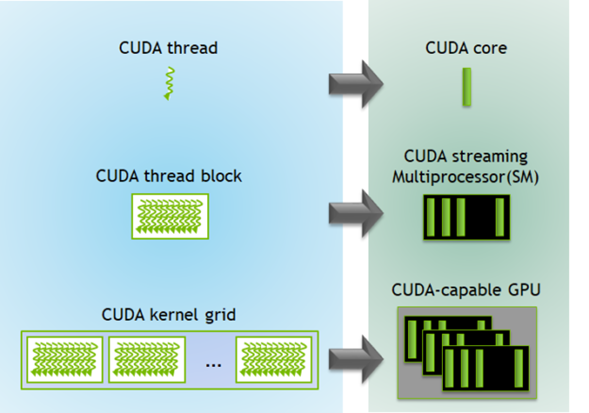
\includegraphics[scale= 0.6]{CUDA.png}
\caption{CPU performance with floats}
\end{figure}



\section{Implementation and reults}
Taking all of the previous information into account the objective was to successfully perform the matrix matrix multiplication in the GPU and improve the performance achieved by the best implementation in the CPU.
\subsection{CPU implementation}
For the CPU implementation, the techniques of unrolling, loop reordering, tiling and threading were used in order to improve the performance of the basic implementation. The results were measured for floating point numbers as well as for double precision and compared with one of the most sophisticated libraries in this type of programming OpenBlas. The measurements obtained can be visualized if the figure 2 and 3 :

\begin{figure}[h]
\centering
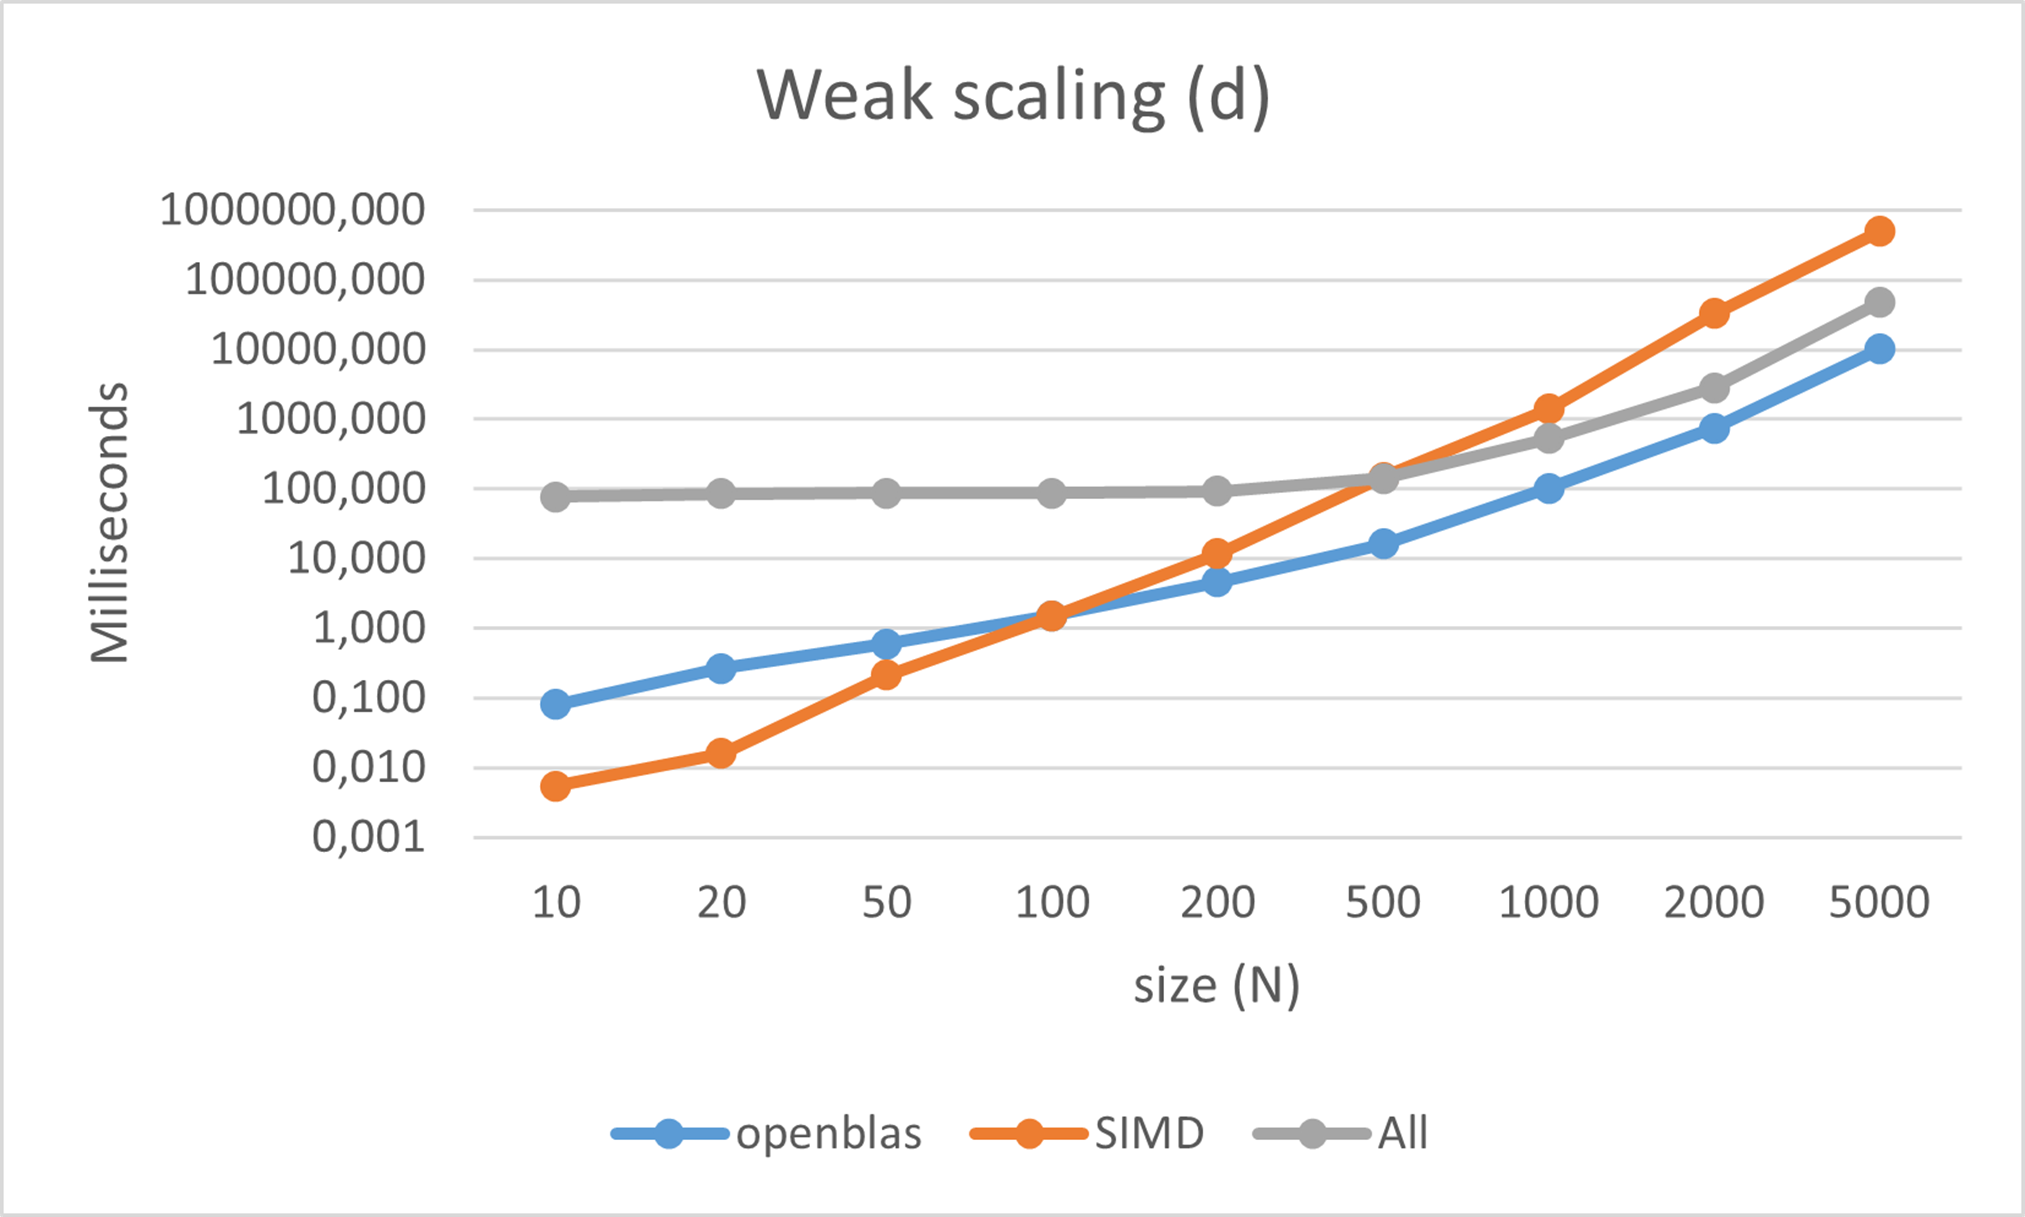
\includegraphics[scale= 0.55]{CPUd.png}
\caption{CPU performance with doubles}
\end{figure}
\begin{figure}[h]
\centering
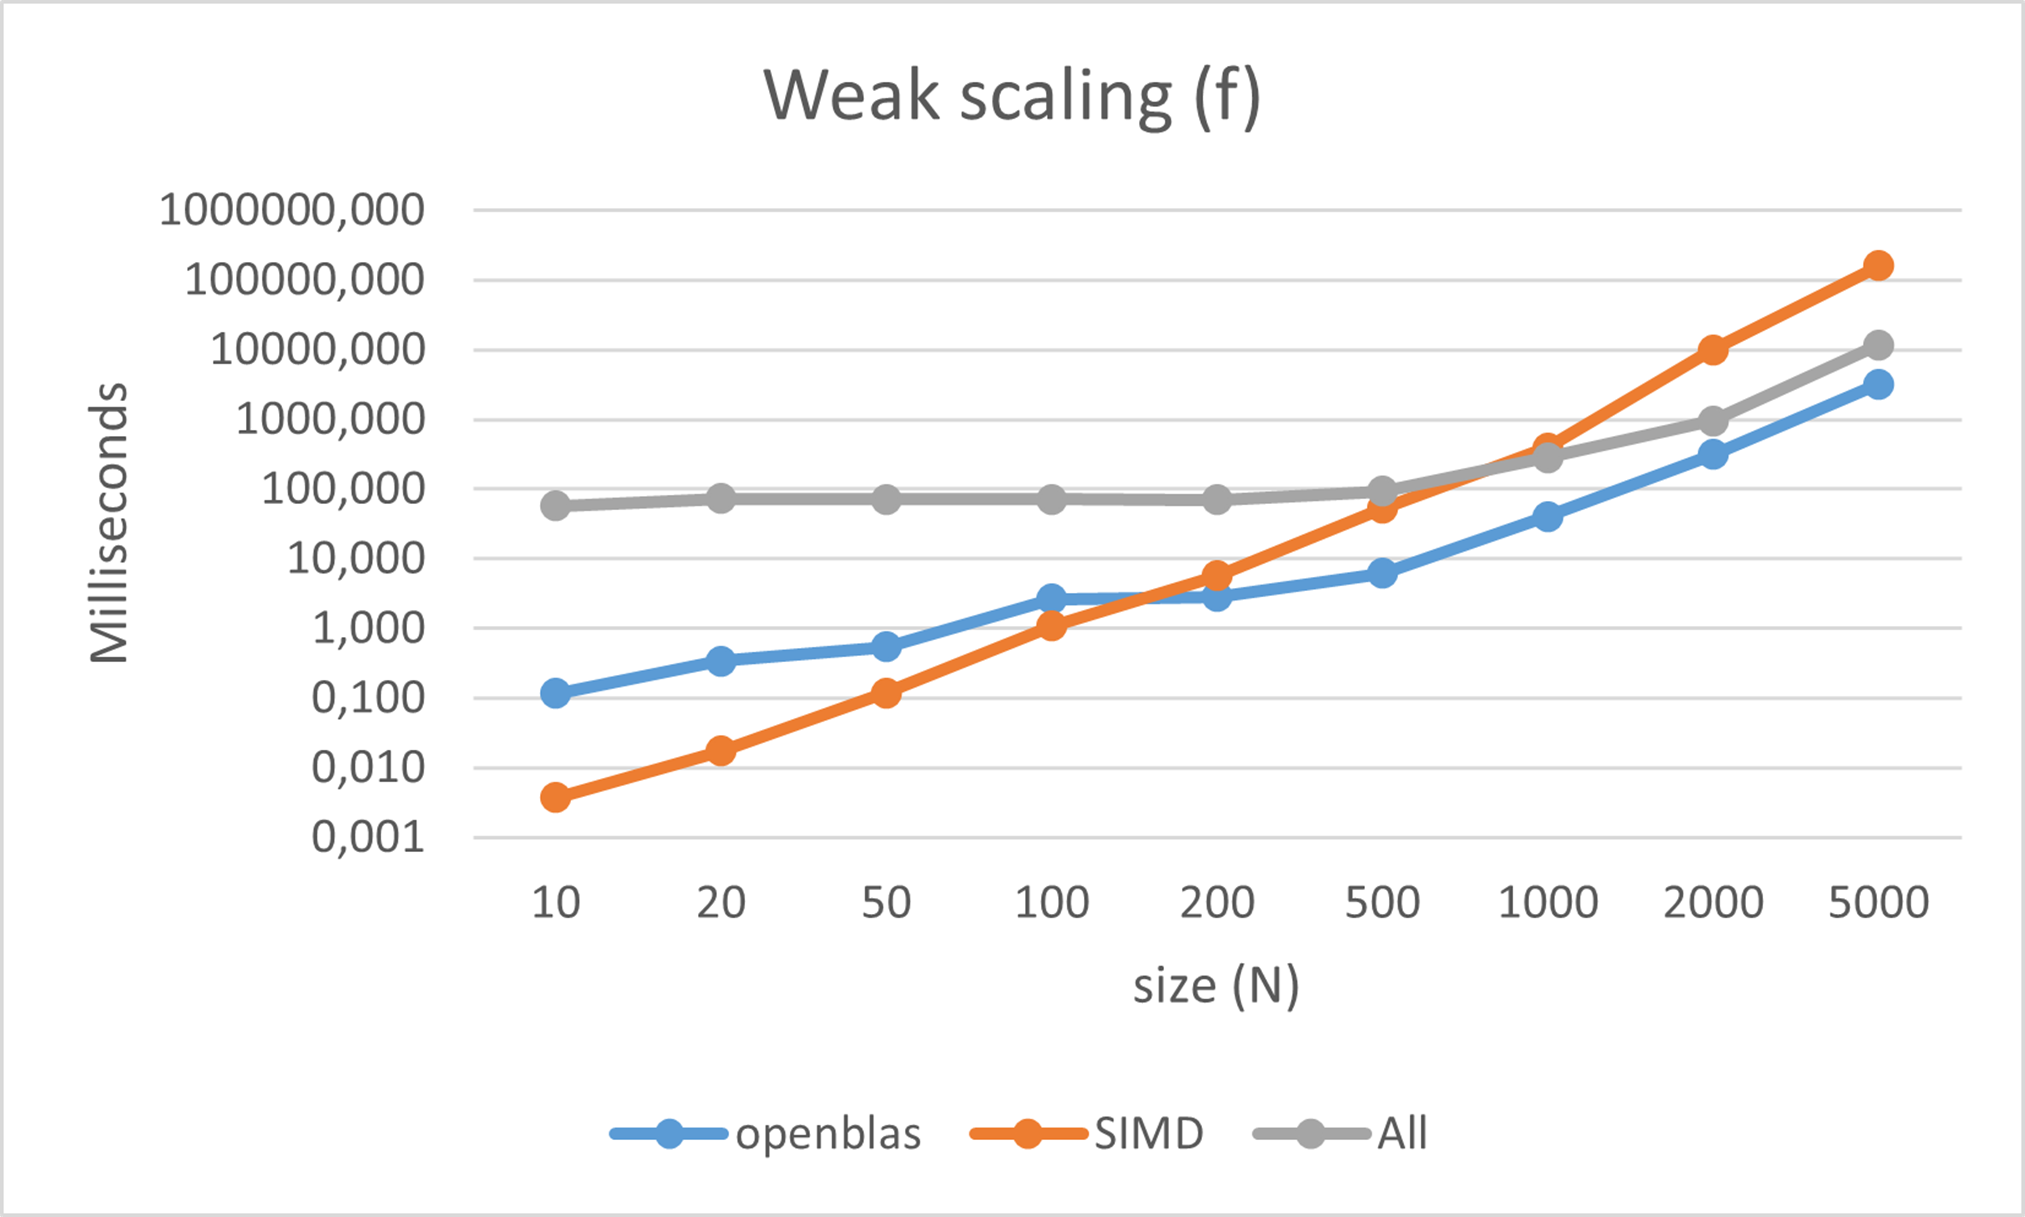
\includegraphics[scale= 0.55]{CPUf.png}
\caption{CPU performance with floats}
\end{figure}

\newpage

\subsection{GPU implementation}
\subsubsection{Block Sizing and Memory Management }
Taking into account the importance of the block size in the performance this implementation might have, the first approach to find an efficient implementation for this method was evaluating which size of block was the most appropriate to perform this operation and evaluate the impact it has. Taking this into account multiple trials with different block sizes and different matrix dimensions were performed. 

Another important aspect when programming in CUDA is the data transfer and memory management.Manually managing memory involves explicitly allocating and deallocating memory on both the CPU and GPU using functions like cudaMalloc and cudaFree. Data transfers between the CPU and GPU must be carefully orchestrated by the programmer, introducing additional complexities and potential sources of error.

Unified Memory Management (UMM), introduced in CUDA 6.0 and later versions, simplifies this process by providing a unified address space accessible by both the CPU and GPU. With UMM, developers no longer need to manually allocate and transfer data between host and device memory; instead, the system automatically handles data movement based on demand. This simplification leads to more concise and readable code, as programmers can focus on the algorithm's logic rather than intricate memory management details.

Despite its advantages UMM might affect performance therefore test were also made comparing these two options.



\subsubsection{Tiling}

The tiling technique in matrix-matrix multiplication is a strategy aimed at improving the efficiency of GPU computations by enhancing memory access patterns and optimizing data locality. Also known as loop blocking or loop tiling, this technique involves breaking down the input matrices into smaller submatrices, called tiles, and performing matrix multiplication on these tiles. By processing smaller tiles that fit into the GPU's cache, the tiling technique helps reduce memory access latency and enhances data reuse, leading to improved overall performance. Tiling allows for better exploitation of parallelism by efficiently utilizing the GPU's parallel processing capabilities. The dimensions of the tiles are carefully chosen to align with the GPU architecture, optimizing memory access patterns and minimizing global memory transactions. In summary, the tiling technique is a powerful optimization strategy in GPU matrix multiplication, enhancing parallelism and minimizing memory access latency to achieve more efficient and accelerated computations.

\begin{figure}[h]
\centering
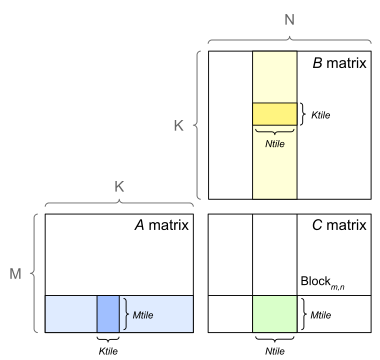
\includegraphics[scale= 0.55]{tiled-outer-prod.png}
\caption{Tiling Matrix Matrix Multiplication}
\end{figure}

\newpage

\subsection{Results}

To implement the previous strategies and testing a NVIDIA Testla T4 GPU was used with the computing power provided by the Google Colaboratory tool. This GPU has the following properties:
\begin{itemize}
    \item Max Blocks Per MultiProcessor: 16 
    \item Max Threads Per MultiProcessor: 1024
    \item Max Threads Per Block: 1024
    \item Number SM: 40
    \item Number bytes sharedMem Per Block: 49152
    \item Number bytes sharedMem Per Multiprocessor: 65536
    \item Memory Clock Rate (KHz): 5001000
    \item Memory Bus Width (bits): 256
    \item Peak Memory Bandwidth (GB/s): 320.064000 
\end{itemize}  
Implementing the previous strategies the following results were obtained:

\medskip
\medskip

Multiple matrix sizes and block sizes with Manual Memory Management:
\begin{figure}[H]
\centering
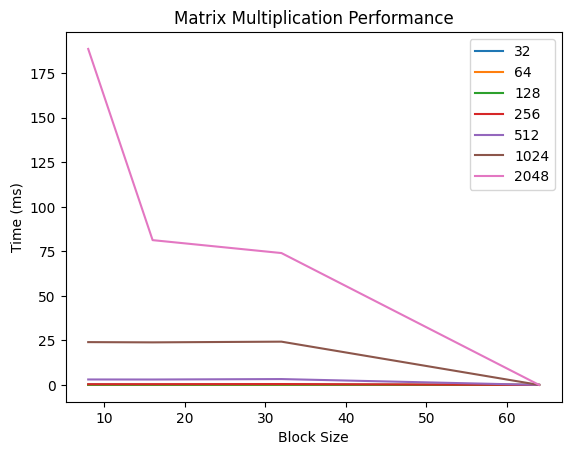
\includegraphics[scale= 0.6]{ManualS.png}
\caption{Manual Memory Management n = [32,2048]}
\end{figure}

\begin{figure}[H]
\centering
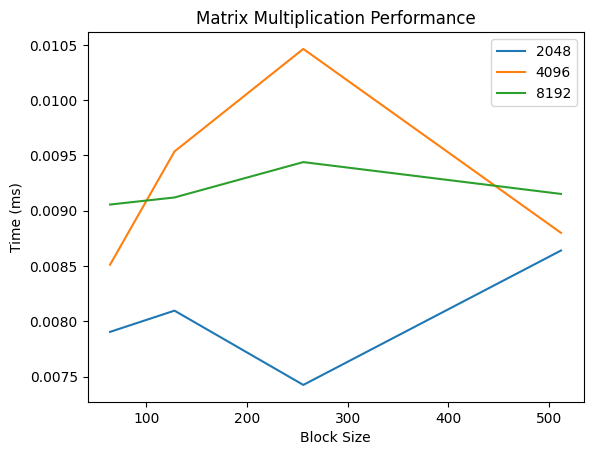
\includegraphics[scale= 0.6]{ManualL.png}
\caption{Manual Memory Management n = [2048,16384]}
\end{figure}

Multiple sizes and block sizes with Unified Memory Management:
\begin{figure}[H]
\centering
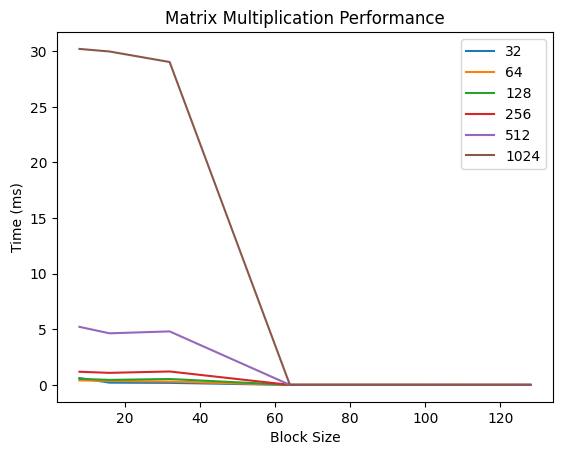
\includegraphics[scale= 0.6]{UnifiedS.png}
\caption{Unified Memory Management n = [32,2048]}
\end{figure}

\begin{figure}[H]
\centering
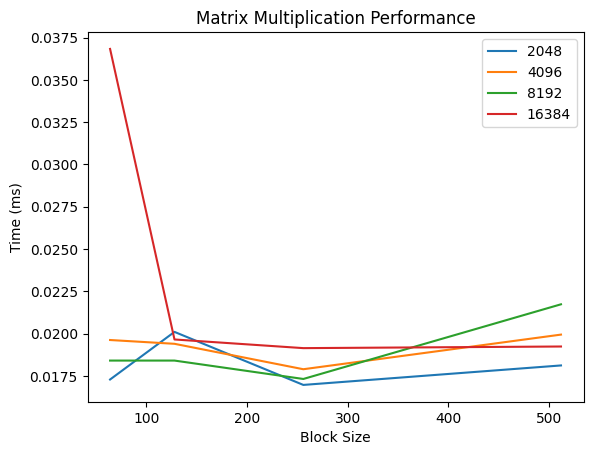
\includegraphics[scale= 0.6]{UnifiedL.png}
\caption{Unified Memory Management n = [2048,16384]}
\end{figure}

\begin{figure}[H]
\centering
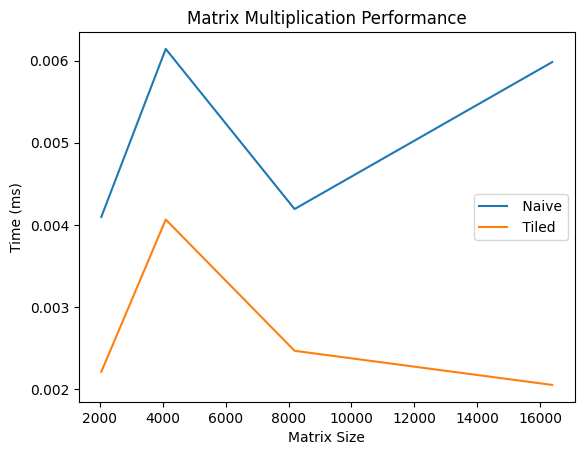
\includegraphics[scale= 0.6]{TiledL.png}
\caption{Tiled vs Naive Comparison n = [2048,16384]}
\end{figure}

\begin{table}
    \centering
    \begin{tabular}{|c|cc|}
    \hline
        \textbf{MatrixSize} & \textbf{Technique} & \textbf{Time} \\ \hline
        2048 & Naive & 0.004096 \\ 
        2048 & Tiled & 0.002208 \\ 
        4096 & Naive & 0.006144 \\ 
        4096 & Tiled & 0.004064 \\ 
        8192 & Naive & 0.004192 \\ 
        8192 & Tiled & 0.002464 \\ 
        16384 & Naive & 0.005984 \\ 
        16384 & Tiled & 0.002048 \\ \hline
    \end{tabular}
    \caption{Technique comparison}
\end{table}

\newpage

\section{Conclusions}

With the previous results we can see the impact and outstanding performance it can be achieved with the utilization of the GPUs computational power. Matrix-Matrix multiplications of dimensions that were previously not feasible were not only performed but also achieved excellent results. It can also be seen how the choice of the block size may have on the performance of this operation, and the effectiveness of the tiling technique that allows to use the resources provided by the GPU in an effective way. 


\end{document}
